\documentclass[
aspectratio=169,
usenames,
dvipsnames,
8pt
% handout
]{beamer}
% \usepackage[dvipsnames]{xcolor}
\usepackage[utf8]{inputenc}
\usepackage{amsmath}
\usepackage{setspace}


\usepackage{subcaption}
\usepackage{mycommands}
\usepackage{nicefrac}
\usepackage{listings}

\usepackage{graphicx,array}


\captionsetup[subfigure]{labelformat=empty}

% \usepackage[numbers]{natbib}

% \usepackage[sorting=none]{biblatex}

\newcolumntype{C}[1]{>{\centering\let\newline\\\arraybackslash\hspace{0pt}}m{#1}}
\newcolumntype{L}[1]{>{\raggedright\let\newline\\\arraybackslash\hspace{0pt}}m{#1}}
\newcolumntype{R}[1]{>{\raggedleft\let\newline\\\arraybackslash\hspace{0pt}}m{#1}}

\graphicspath{{../written/thesis/figma-illustrations/},{../written/thesis/symlinks/illustrations},{../written/thesis},{../written/thesis/symlinks/zero-one-plots}}



\newcommand{\twg}[1]{
  \begin{figure}
    \centering
    \includegraphics[width=\textwidth]{#1}
  \end{figure}
}
\newcommand{\twgc}[2]{
  \begin{figure}
    \centering
    \includegraphics[width=\textwidth]{#1}
    \caption{#2}
  \end{figure}
}

% https://tex.stackexchange.com/questions/102069/make-a-heading-in-beamer
\newcommand\myheading[1]{%
  \par\bigskip
  {\large#1}\par\smallskip}
\newcommand\hd[1]{\myheading{#1}}

% https://tex.stackexchange.com/a/388900
\setbeamertemplate{itemize item}[circle]

\newcommand{\thirdcol}{\column{0.3\textwidth}}
\newcommand{\twothirdcol}{\column{0.6\textwidth}}
\newcommand{\fourthcol}{\column{0.25\textwidth}}
\newcommand{\halfcol}{\column{0.5\textwidth}}
\newcommand{\seventhcol}{\column{0.7\textwidth}}

\newcommand{\papertitle}[1]{
  \centering
  \textcolor{BlueViolet}{
    #1
  }
  \\
}

\newcommand{\paperauthors}[1]{
  \footnotesize
  \centering
  \textcolor{gray}{
    \textit{
      #1
    }
  }
  \\
}

% \captionsetup{font=scriptsize}
\usepackage[labelformat=empty,font={color=gray,scriptsize},justification=centering]{caption}

% \setbeamertemplate{page number in head/foot}{\insertframenumber}
% \setbeamertemplate{footline}{\raggedleft \raisebox{1.8pt}[0pt][0pt]{\insertframenumber}}

\setbeamertemplate{navigation symbols}{}%remove navigation symbols

\addtobeamertemplate{navigation symbols}{}{ \hspace{1em}    \usebeamerfont{footline}%
  \insertframenumber}


% \usepackage{fontspec}

\usepackage{tikzsymbols}




% black accent color
\usecolortheme[named=black]{structure}


% less prominent frametitle stuff stuff
\setbeamercolor{frametitle}{fg=black!75}
\setbeamerfont{frametitle}{size=\small}

\setbeamertemplate{frametitle}[default][center]


% box styling
% 1- Block title (background and text)
\setbeamercolor{block title example}{fg=white, bg=teal}
\setbeamercolor{block body example}{bg=teal!25}

\newenvironment<>{definitionblock}[1]{%
  \setbeamercolor{block title}{fg=black,bg=def}%
  \setbeamercolor{block body}{bg=def}%
  \setbeamercolor{item}{fg=black}
  \begin{block}#2{\small\textbf{#1}}}{\end{block}}

\newenvironment<>{questionblock}[1]{%
  \setbeamercolor{block title}{fg=black,bg=ques}%
  \setbeamercolor{block body}{bg=ques}%
  \setbeamercolor{item}{fg=black}
  \begin{block}#2{\small\textbf{#1}}}{\end{block}}

\newenvironment<>{theoremblock}[1]{%
  \setbeamercolor{block title}{fg=black,bg=thm}%
  \setbeamercolor{block body}{bg=thm}%
  \setbeamercolor{item}{fg=black}
  \begin{block}#2{\small\textbf{#1}}}{\end{block}}

\newenvironment<>{corollaryblock}[1]{%
  \setbeamercolor{block title}{fg=black,bg=cor}%
  \setbeamercolor{block body}{bg=cor}%
  \setbeamercolor{item}{fg=black}
  \begin{block}#2{\small\textbf{#1}}}{\end{block}}

\newenvironment<>{objectiveblock}[1]{%
  \setbeamercolor{block title}{fg=white,bg=Bittersweet!35}%
  \setbeamercolor{block body}{bg=Bittersweet!10}%
  \setbeamercolor{item}{fg=Bittersweet!35}
  \begin{block}#2{#1}}{\end{block}}


\newenvironment<>{resultblock}[1]{%
  \setbeamercolor{block title}{fg=white,bg=teal}%
  \setbeamercolor{block body}{bg=teal!25}%
  \setbeamercolor{item}{fg=teal}
  \begin{block}#2{#1}}{\end{block}}


\newenvironment<>{observationblock}[1]{%
  \setbeamercolor{block title}{fg=white,bg=gray}%
  \setbeamercolor{block body}{bg=gray!25}%
  \setbeamercolor{item}{fg=gray}
  \begin{block}#2{#1}}{\end{block}}



% Information to be included in the title page:
\title{Model Correlation in Random Forests}
\author{}
\date{}
\institute{}


\newcommand{\colandmargin}[2]{
  \begin{columns}
  \begin{column}{0.66\textwidth}
    #1
  \end{column}
  \begin{column}{0.33\textwidth}  %%<--- here
      \begin{center}
        #2
      \end{center}
  \end{column}
  \end{columns}
}


\usepackage{amsmath}
% \usepackage{unicode-math}
\usepackage{../written/thesis/preamble}
%\usepackage{bbm}
\usepackage{unicode-math}
\renewcommand{\ind}[1]{\mathbb{1}\left[#1\right]}


% \usepackage[sorting=none]{biblatex}
% \addbibresource{../written/thesis/symlinks/zotero-library-automatic-export.bib}

\begin{document}

\frame{\titlepage} 

\begin{frame}
    \centering
    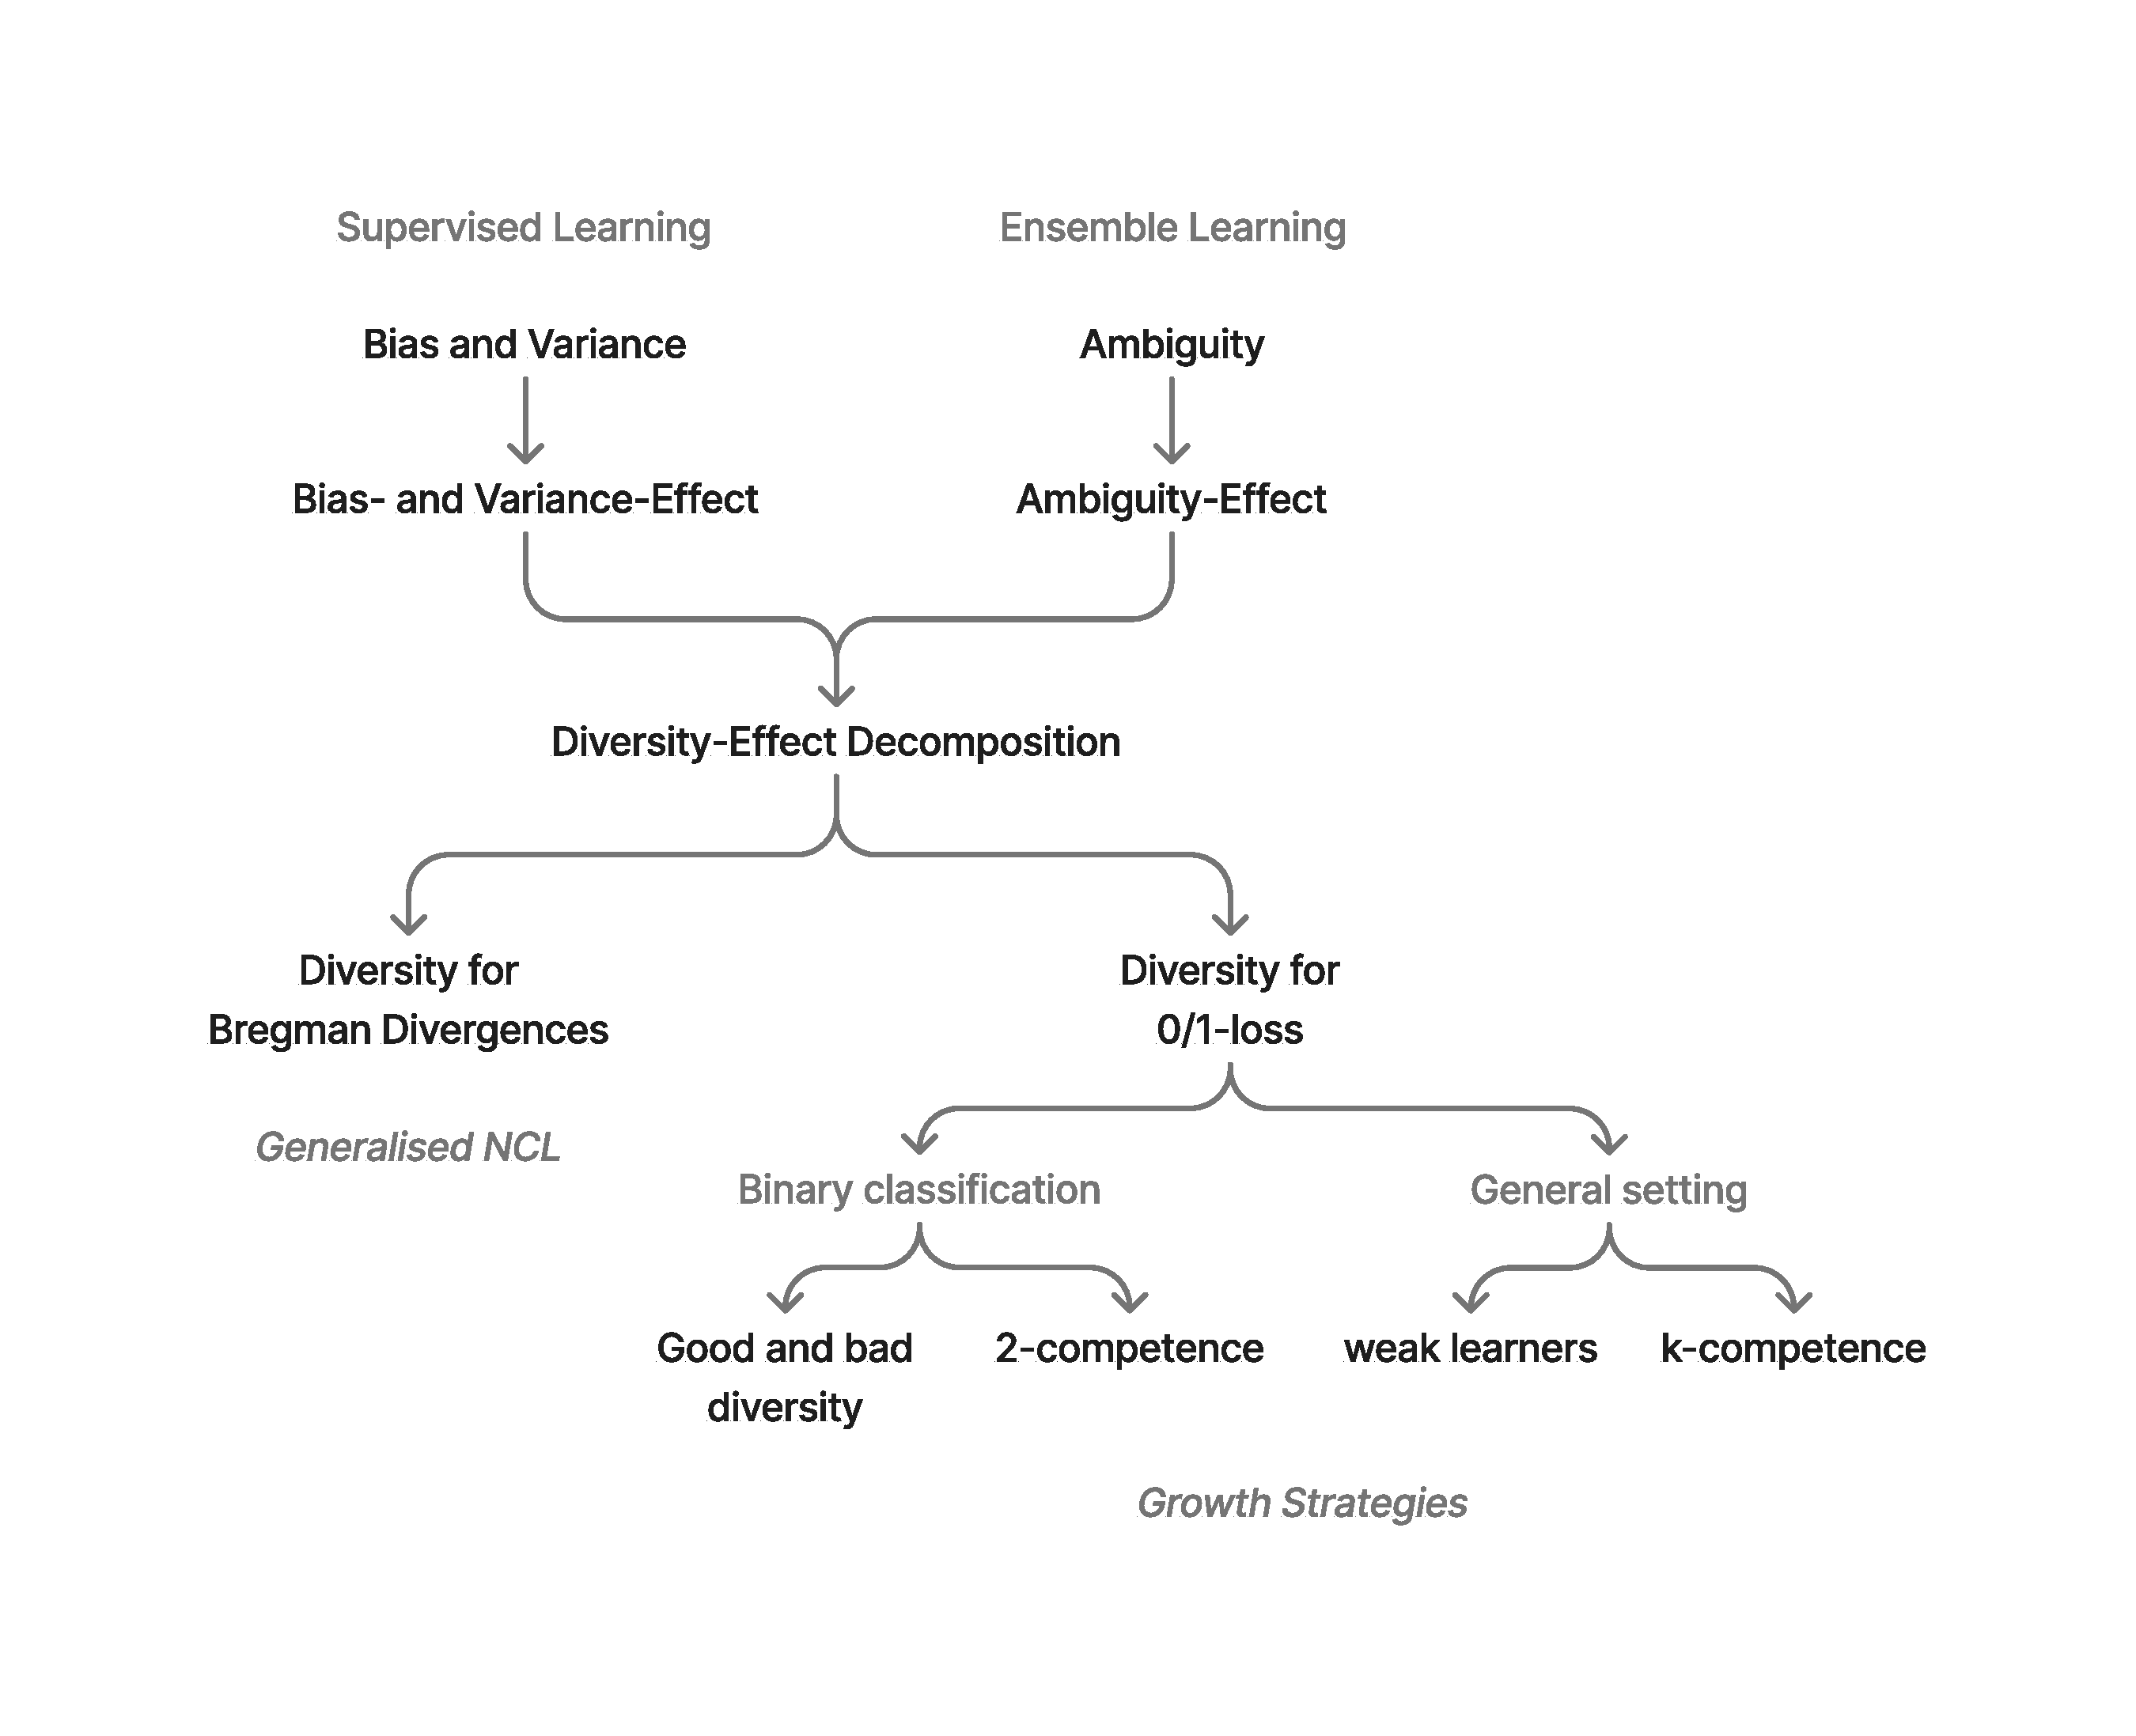
\includegraphics[width=0.8\textwidth]{figma-illustrations/thesis-overview.pdf}
\end{frame}

% \section{foo}

\begin{frame}

  \begin{questionblock}{Supervised Learning objective}
    \begin{itemize}
      \item Given features (description) of an object, predict an outcome for it.
      \item How to predict? Based on set of examples which we already know the outcome.
      \item Infer abstract \textit{model} of unknown data from known training data
      \item[$\rightarrow$] Find a learning algorithm $\mathcal{A}$ that can be expected to produce "good" models.
    \end{itemize}
  \end{questionblock}

  \begin{corollaryblock}{Application example: Virtual Screening}
  % https://www.ncbi.nlm.nih.gov/pmc/articles/PMC3018816/
  \begin{itemize}
    \item Many different cancer cell lines tested for their response to certain drugs
    \item Predict drug response for new cell lines
  \end{itemize}
  Determine promising candidates for more expensive \textit{in-vitro} screening.
  \end{corollaryblock}

  We need:
  \begin{itemize}
    \item Language and measures to assess learning algorithms
  \end{itemize}

  % 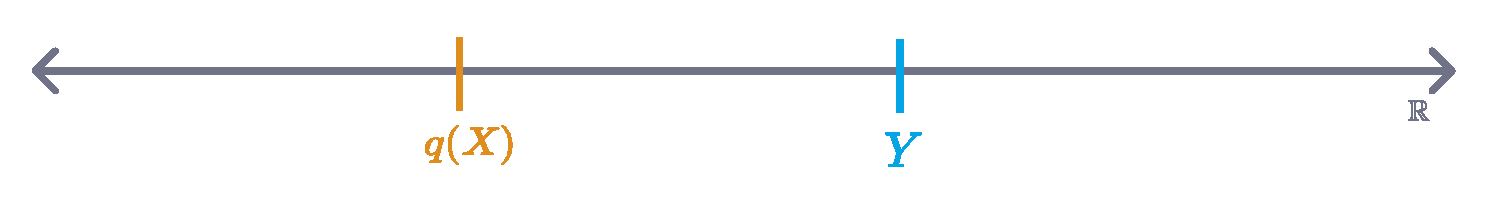
\includegraphics[width=\textwidth]{lnl-loss}

\end{frame}

\begin{frame}

  % examples for different loss functions...

  \colandmargin{


{\large
\begin{align*}
  \text{Setup}: &\hspace{1em}   D \sim P( \underset{\text{Features} }{\mathcal{X}}, \underset{\text{Outcomes} }{\mathcal{Y}} )^n
\\[2em]
\text{Training}: &\hspace{1em} \underset{\text{Input}}{D} ~\rightarrow~ \underset{\text{Learner} }{\mathcal{A}} ~\rightarrow~ \underset{\text{Model} }{q_{D}} \\[2em]
\text{Evaluation:}  &\hspace{1em} (X,Y) \sim P(\mathcal{X}, \mathcal{Y}); ~ ~ \ell(q_{D}(X), Y)
\end{align*}
}
  }{

    \begin{definitionblock}{Loss / Error}
      Function $\ell: \mathcal{Y} \times \mathcal{Y} \to \mathbb{R}_+$ to assess the error between two outcomes (e.g. true and predicted).
    \end{definitionblock}

    \begin{definitionblock}{Model}
      Function $q: \mathcal{X} \to \mathcal{Y}$. In supervised learning, the model depends on the training input $D$. Model prediction:   $$
      q_{D}(X)
      $$
    \end{definitionblock}
  }


  \colandmargin{


    \begin{definitionblock}{ Risk and Generalisation Error }
    The \textit{risk} of a model $q_D$ is the expected loss over all example-outcome pairs.
    $$
    \text{Risk}(q_{D}) \defeq \mathbb{E}_{(X,Y)\sim P}\left[ \ell(Y, q_{D}(X)) \right] 
    $$
    %
    The quality of a given learning algorithm $\mathcal{A}$ is the expected risk over all possible inputs $D$. We refer to this as the \textit{generalisation error}. 
    $$
    \text{GE}(\mathcal{A}) \defeq \mathbb{E}_{D}\left[ \text{Risk}(q_{D}) \right]  = \mathbb{E}_{(X,Y), D}\left[ \ell(Y, q_{D}(X)) \right] 
    $$
    \end{definitionblock}

  }{
    \small
    \begin{itemize}
      \item Risk is property of model
      \item Generalisation error is property of learner
    \end{itemize}
  }
\end{frame}

\begin{frame}

  \colandmargin{
    Basic idea: model prediction should be guided by outcomes of "similar" training examples.

    \begin{definitionblock}{Decision Tree learner}
      \begin{itemize}
        \item Recursively perform binary splits in feature space $\mathcal{X}$
        \item Split such that "purity" of outcomes in cell is improved
        \item To predict, use centroid prediction of training examples in cell
      \end{itemize}
    \end{definitionblock}

    \begin{corollaryblock}{}
      Prediction is cell-wise constant
    \end{corollaryblock}

  }{
    \centering
    \includegraphics[width=0.7\textwidth]{tree-partition}
    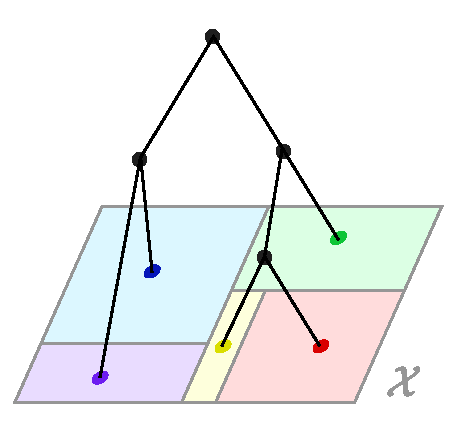
\includegraphics[width=0.7\textwidth]{decision-tree}
  }
\end{frame}

\begin{frame}
  \centering
  \includegraphics[width=0.8\textwidth]{decision-trees/penguins-a}
\end{frame}

\begin{frame}
  \centering
  \includegraphics[width=0.8\textwidth]{decision-trees/penguins-b}
\end{frame} 

\begin{frame}
  
  \frametitle{
    Components of error for single point $(X,Y)$
  }

  \colandmargin{
    \centering
    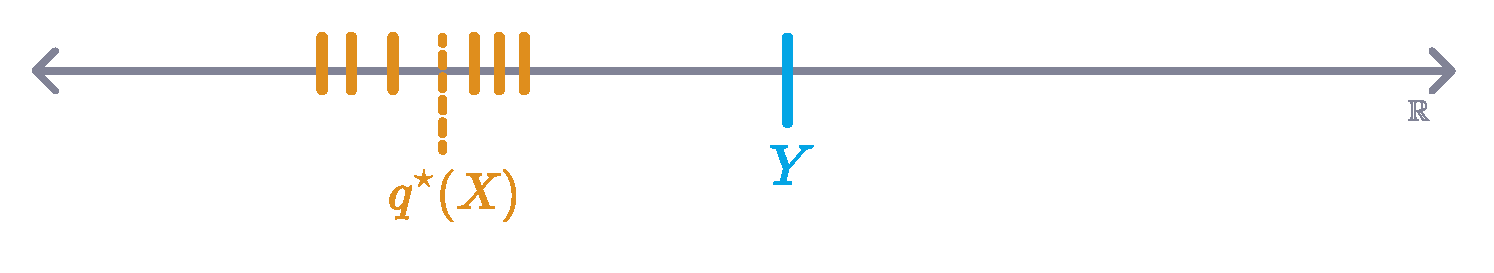
\includegraphics[width=\textwidth]{lnl-bias-nonoise}
    {\small
    $\text{bias}(X,Y) \defeq \ell(Y, q^\star)$
    }
  }{
    \begin{definitionblock}{Central Model}
    $$
    q^\star \defeq \arg\min_{z} \mathbb{E}_{D}\left[ \ell(z, q_{D}) \right] 
    $$
    \end{definitionblock}
  }

  \vspace{2em}

  \colandmargin{
    \centering
    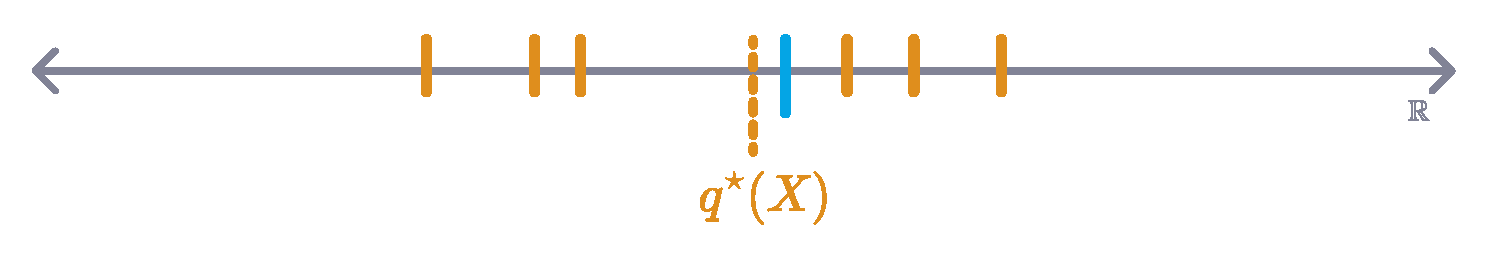
\includegraphics[width=\textwidth]{lnl-variance}
    {\small
      \begin{align*}
        \text{variance-effect}(X,Y) &\defeq \mathbb{E}_D \left[ \ell(Y, q_D)  \right] - \ell(Y, q^\star) \\
        &= \mathbb{E}_D \left[ \ell(Y, q_D) - \ell(Y, q^\star)   \right]  \\
        &= \mathbb{E}_D \left[ \LE{q^\star}{q_D} \right]
      \end{align*}
    }
  }{
    \begin{definitionblock}{Loss-Effect} For a loss functon $\ell$, and random variables $Y, Z, Z'$, we define the change in loss between $Z$ and $Z'$ in relation to $Y$ as:
      $$
      \LE{Z}{Z'} \defeq \ell(Y, Z') - \ell(Y, Z)
      $$
    \end{definitionblock}
  }

\end{frame}


\begin{frame}


  \begin{theoremblock}{Bias-Variance-Effect-Decomposition for single point $(X,Y)$ (no noise)  }
    \label{thm:bias-variance-effect}
    For any loss function $\ell$, it holds that
    \begin{align*}
    \mathbb{E}_{D}\left[ \ell(Y, q_{D}) \right]  
    &= 
    \ell(Y, q^\star) + 
    \mathbb{E}_D \left[ \ell(Y, q_D) - \ell(Y, q^\star)   \right]  \\
    &= 
    % \underbrace{\mathbb{E}_{(X,Y)}\left[ \ell(Y, y^\star) \right]  }_{\text{noise}} + 
    % \underbrace{\LE{Y}{q^\star}}_{\text{bias}}
    \underbrace{\ell(Y, q^\star)}_{\text{bias}}
    + \underbrace{\mathbb{E}_{D}\left[ \LE{q^\star}{q_D} \right] }_{\text{variance-effect}}  \\
    % \\ 
    % \text{for} \hspace{1em}
    % & \LE{q^\star}{y^\star} = \ell(Y, q^\star) - \ell(Y, y^\star) \\ \\
    % &\LE{q^\star}{q_D} = \ell(Y, q_{D}) - \ell(Y, q^\star)
    \end{align*}
  \end{theoremblock}

For the squared-error loss $\ell(Z, Z') = (Z - Z')^2$, variance-effect = variance.
% $$
%  \mathbb{E}_{}\left[ \ell(Y, q^\star) - \ell(Y, y^\star) \right]  = \mathbb{E}_{}\left[ \ell(y^\star, q^\star) \right]
% $$
$$
 \mathbb{E}_{}\left[ \ell(Y,q) - \ell(Y, q^\star) \right]  = \mathbb{E}_{}\left[ \ell(q^\star, q)  \right] 
$$
\end{frame}


\begin{frame}

  \frametitle{Interpolation and Bias-Variance-Tradeoff}

  % so let's see how decision trees do, ...

  \colandmargin{
    \centering
    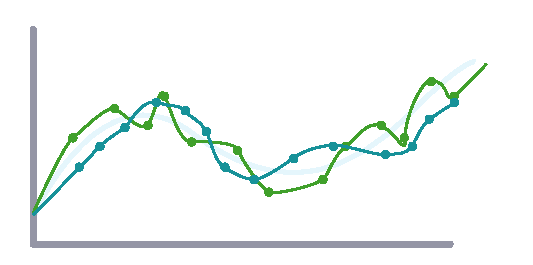
\includegraphics[width=0.7\textwidth]{bias-variance-tradeoff-a}
    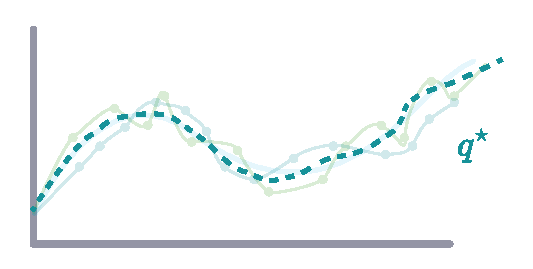
\includegraphics[width=0.7\textwidth]{bias-variance-tradeoff-b}
    % note q^star is the central/expected model, never a real model that we get
  }{
    \begin{figure}
    \includegraphics[width=\textwidth]{bias-variance/bias_variance_decomposition_with_decision_trees.png}
    \caption{Bias and variance of decision tree models of increasing maximum tree depth. With increasing tree depth, \tcircle{orange} bias tends to decrease, as \tcircle{green} variance tends to increase.}
    \end{figure}
  }

  \begin{corollaryblock}{}
    Deep decision trees achieve low bias, but have high variance.
  \end{corollaryblock}

  % one idea: limit tree depth

  % another idea: averaging, (i.e. imitate q^star) <- this might be more misleading than helpful though
  % elimiate strong dependence on realisation of D

\end{frame}


\begin{frame}

  \colandmargin{
    A Random Forest is an ensemble of $M$ \textbf{randomised} decision trees.

    \begin{definitionblock}{}
    Member learner (randomized with RV $\Theta$, for e.g. single tree in forest)
      $$
      \mathcal{A}_{\text{DT}}(D, \Theta) ~ ~ \leadsto ~ ~ q_{D, \Theta} : \mathcal{X} \to \mathcal{Y}
      $$
    \end{definitionblock}

  }{
    \small Randomness $\Theta$ used for
    \begin{itemize} \small
      \item Construct tree on random subset of $D$
      \item Only consider random subsample of feature dimensions for split search
    \end{itemize}
  }

  \colandmargin{

    \begin{definitionblock}{}
    Random Forest learner 
    $$
    \mathcal{A}_{\text{RF} }(D) ~ ~ \leadsto ~ ~  \bar{q}_{D}: \mathcal{X} \to \mathcal{Y} : x \mapsto \arg \min_{z} \mathbb{E}_{\Theta}\left[ \ell(z, q_{D,\Theta}(x)) \right] 
    $$
    \end{definitionblock}
    {\small
      Implementation of $\mathcal{A}_{\text{RF}}$: 
      \begin{itemize}
        \item Given $D$, repeat
        \begin{enumerate}
          \item Draw $\Theta$
          \item Construct a tree $q_{D, \Theta} \gets \mathcal{A}_{\text{DT}}(D, \Theta)$
        \end{enumerate}
        \item  return $\bar{q}_{D} = \arg \min_{z} \mathbb{E}_{\Theta}\left[ \ell(z, q_{\Theta}) \right]$
      \end{itemize}
    }


  }{
    \small
    $$
       D \sim P( \underset{\text{Features} }{\mathcal{X}}, \underset{\text{Labels} }{\mathcal{Y}} )^n
    $$
    $$
     \underset{\text{Input}}{D} ~\rightarrow~ \underset{\text{Learner} }{\mathcal{A}} ~\rightarrow~ \underset{\text{Model} }{q_{D}} 
    $$
  }

\end{frame}

\begin{frame}
  \begin{figure}
  \includegraphics[width=\textwidth]{decision-trees/penguins-forest-individual}
  \caption{Trees constructed using 3 different realisations of $\Theta$. Scattered points are the bootstrap samples of $D$.}
  \end{figure}
\end{frame}

\begin{frame}
  \colandmargin{

  \centering
  \includegraphics[width=0.65\textwidth]{decision-trees/penguins-forest-combined} 
  }{}

  \colandmargin{
  \begin{definitionblock}{Ensemble Combiner}
   The ensemble combiner $\bar{q} : \mathcal{X} \to \mathcal{Y}$ for a given loss function $\ell$ is the centroid with respect to model parameters $\Theta$: 
  $$
  \bar{q} \defeq \arg\min_z \mathbb{E}_\Theta \left[ \ell(z, q_\Theta) \right]
  $$
  \end{definitionblock}
  }{
  \small
  \begin{itemize}
    \item squared-error-loss: $\bar{q} = \mathbb{E}_\Theta\left[q_\Theta\right] \approx \Mavg q_i$
    \item \zeroone-loss: $\bar{q}$ is plurality vote
    \item $\bar{q}$ is central model w.r.t. distribution of member parameters $\Theta$
  \end{itemize}

  }
\end{frame}


\begin{frame}
  \colandmargin{
  
  \begin{itemize}
    \item The Random Forest learner has lower variance than the decision tree learner
    \item ... while bias is not affected "too much"
  \end{itemize}
  \vspace{2em}
  \begin{questionblock}{Questions}
    \begin{itemize}
      \item When and why do such ensemble techniques work?
      \item In particular, what makes Random Forests work so well?
    \end{itemize}
  \end{questionblock}
  }{
    \centering
    \includegraphics[width=0.7\textwidth]{bias-variance/test_error_of_individual_trees.png}
  }
\end{frame}

\begin{frame}
  % Ambiguity-effect decomp

    \begin{definitionblock}{Ensemble Improvement / Diversity-Effect} The \textit{ensemble improvement} is the difference in loss between the ensemble combiner and an average member.
    $$
    \mathbb{E}_{\Theta}\left[   \ell(Y, q_{\Theta})  \right]  -  \ell(Y, \bar{q}))
    = \mathbb{E}_{\Theta} \left[ \LE{\bar{q}}{q_\Theta} \right] 
    % \approx \Mavg \ell(Y, q_i) - \ell(Y, \bar{q})
    $$
    \end{definitionblock}

    {
    \small
    \begin{align*}
      \text{variance-effect}(X,Y) &\defeq 
    \mathbb{E}_D \left[ \LE{q^\star}{q_D}   \right] 
    & q^\star \defeq \arg\min_{z} \mathbb{E}_{D}\left[ \ell(z, q_{D}) \right] 
    \\[1em]
    \text{diversity-effect}(X,Y) &\defeq 
    \mathbb{E}_\Theta \left[ \LE{\bar{q}}{q_\Theta}   \right] 
    & 
    \bar{q} \defeq \arg\min_z \mathbb{E}_\Theta \left[ \ell(z, q_\Theta) \right]
    \end{align*}
    }

  \begin{theoremblock}{ Ambiguity-Effect decomposition } For any loss function $\ell$, target label $Y$, ensemble members $q_{1}, \dots, q_{M}$ with combiner $\bar{q}$
  \begin{align*}
  \ell(Y, \bar{q})
  &= \mathbb{E}_{\Theta}\left[ \ell(Y, q_{\Theta}) \right] - \mathbb{E}_{\Theta}\left[ \ell(Y, q_{\Theta}) - \ell(Y, \bar{q}) \right] \\
  &= \mathbb{E}_{\Theta}\left[ \ell(Y, q_{\Theta}) \right]  - \mathbb{E}_{\Theta}\left[ \LE{\bar{q}}{q_{\Theta}} \right] \\
  \end{align*}
  \end{theoremblock}
  % {\small
  % $$
  % \ell(Y, \bar{q}) \approx \Mavg \ell(Y, q_{i}) -
  % \underbrace{\left(\Mavg \ell(Y, q_{i}) - \ell(Y, \bar{q})\right)}_{\text{Ambiguity-Effect / Ensemble Improvement}} \\
  % $$
  % }

  \begin{corollaryblock}{}
    \textbf{Trade-off between average member error and diversity}
  \end{corollaryblock}



\end{frame}



\begin{frame}

  \colandmargin{
Start with ambiguity decomposition
$$
\mathbb{E}_{D}\left[ \ell(Y, \bar{q}) \right]  
=  
\mathbb{E}_{D, \Theta}\left[ \ell(Y, q) \right] - \mathbb{E}_{D, \Theta }\left[ \LE{\bar{q}}{q} \right] 
$$
... and apply bias-variance decomp. to \textit{member} loss $\ell(Y, q)$
\begin{theoremblock}{ Bias-Variance-Diversity-Effect decomposition  }
\begin{align*}
  \mathbb{E}_{D}\left[ \ell(y, \bar{q}) \right] 
= 
\underbrace{
\mathbb{E}_{\Theta}\left[  \ell(Y, q^\star) \right]
}_{\text{avg. bias} }
+
\underbrace{
\mathbb{E}_{D,\Theta}\left[ \LE{q^\star}{q} \right] 
}_{\text{avg. variance-effect} }
-
\underbrace{
\mathbb{E}_{D, \Theta}\left[ \LE{\bar{q}}{q} \right] 
}_{\text{diversity-effect} }
\end{align*}
\end{theoremblock}
  }{
    (diagram of "double decomp trick" like in wood23)
\centering
      \includegraphics[width=0.8\textwidth]{symlinks/zero-one-plots/bvd-decomps/plot_bvd_standard_rf/mnist_subset/bvd-standard_rf.png}
    }

\begin{itemize} \small
  \item A model $q$ depends on both $D, \Theta$
\item An expected/central model $q^\star = \arg \min_{z} \mathbb{E}_{D}\left[ \ell(z, q) \right]$ depends on $\Theta$ only
\item The combiner  $\bar{q} = \arg \min_{z} \mathbb{E}_{\Theta}\left[ \ell(z, q) \right]$  depends on $D$ only
\end{itemize}

\end{frame}


\begin{frame}{Diversity for Bregman divergences}

  \colandmargin{
    \begin{definitionblock}{{Bregman Divergence}} The Bregman divergence $\Breg{p}{q} : \mathcal{S} \times \mathcal{S}\to \mathbb{R}$ is defined based on a generator function $\phi$ as follows:
  $$
  \Breg{p}{q} \defeq \phi(p) - \phi(q) - \inner{\nabla \phi(q)}{(p-q)}
  $$
  where $\inner{\cdot}{\cdot}$ is the inner product, $\nabla \phi(q)$ is the gradient vector of $\phi$ at $q$ and $\phi: \mathcal{S} \to \mathbb{R}$ is a strictly convex function on a convex set $\mathcal{S} \subseteq \mathbb{R}^k$ such that it is differentiable on the relative interior of $\mathcal{S}$.
  \end{definitionblock}
  }{
    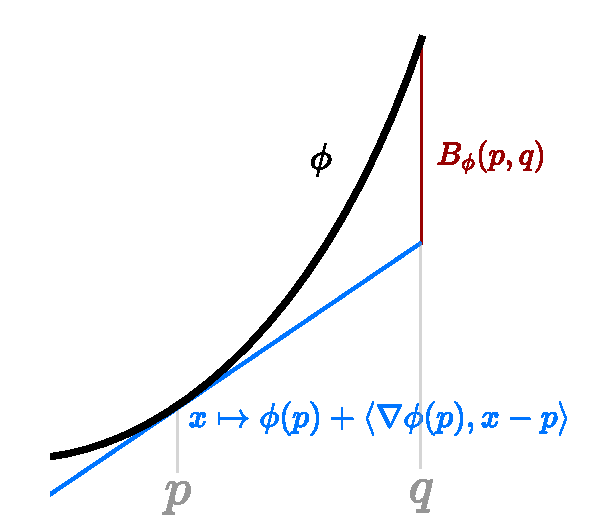
\includegraphics[width=0.8\textwidth]{bregman-div-intuition}
  }

  \vspace{1em}
  {\small
    \begin{tabular}{|l|l|l|l|}
    \hline
        Divergence $\Breg{p}{q}$ & Generator $\phi(q)$ & Domain $S$ & Loss function \\ \hline
        $(p-q)^2$ & $q^2$ & $\mathbb{R}$ & Squared Error \\ \hline
        $p \log \left(\frac{p}{q}\right)+(1-p) \log \left(\frac{1-p}{1-q}\right)$ & $p \log p+(1-p) \log (1-p)$ & $[0,1]$ & Logistic loss \\ \hline
        $\frac{p}{q}-\log \left(\frac{p}{q}\right)-1$ & $-\log p$ & $\mathbb{R}_{>0}$ & Ikura-Saito distance \\ \hline
        $\mid\mid p-q \mid\mid^2$ & $\mid\mid p\mid\mid^2$ & $\mathbb{R}^d$ & Squared Euclidean distance \\ \hline
        $(p-q)^\top A (p-q)$ & $p^\top A q$ & $\mathbb{R}^d$ & Mahalanobis distance \\ \hline
        $\sum_{j=1}^d p_j \log _2\left(\frac{p_j}{q_j}\right)$ & $\sum_{j=1}^d p_j \log _2 p_j$ & $d$-simplex & KL-divergence \\ \hline
        $\sum_{j=1}^d p_j \log \left(\frac{p_j}{q_j}\right)-\sum_{j=1}^d\left(p_j-q_j\right)$ & $\sum_{j=1}^d p_j \log p_j$ & $\mathbb{R}^d_{\geq {0}}$ & Generalized I-divergence \\ \hline
        $\sum_{j=1}^d p_j \log p_j$ & $\sum_{j=1}^d p_j \log p_j$ & $\mathbb{R}_{\geq {0}}$ & Poisson loss \\ \hline
    \end{tabular}
  }

\end{frame}


\begin{frame}
  \begin{theoremblock}{Left and right Bregman centroids}
        Let $B_{\phi}$ be a Bregman divergence of generator $\phi: \mathcal{S} \to \mathbb{R}$. For a random variable $Y$ taking values in $\mathcal{S}$, it holds that
    \begin{itemize}
        \item the \textit{right Bregman centroid} is $$\arg \min_z \mathbb{E}_{X}\left[ \Breg{X}{z}  \right] = \mathbb{E}_{}\left[ X \right]$$
        \item the \textit{left Bregman centroid} is $$\arg\min_{z}  \mathbb{E}_{X}\left[ \Breg{z}{X}\right] = (\nabla \phi)^{-1} \mathbb{E}_{}\left[ \nabla \phi(X) \right] \defeq \mathcal{E}\left[X\right]$$
    \end{itemize}
      If $B_\phi$ is symmetric, i.e. $\Breg{Y}{Y'} = \Breg{Y'}{Y}$ then $\mathbb{E}\left[X\right] = \mathcal{E}\left[X\right]$.
  \end{theoremblock}
\begin{definitionblock}{Dual expectation}
  The left Bregman centroid is the expected value in the dual space implied by $\nabla\phi$. Due to this, we define the dual expectation as  
  $$\mathcal{E}\left[X\right] \defeq (\nabla \phi)^{-1}\mathbb{E}_{}\left[ \nabla \phi(X) \right]$$ 
\end{definitionblock}
For Bregman divergences, $q^\star$ and $\bar{q}$ are left Bregman centroids.
\end{frame}

\begin{frame}
  \begin{theoremblock}{}
  Let $q$ be a function of random variable $Z$ and independent of $Y$. For $q^\star = \mathcal{E}_{Z}\left[ q \right]$, i.e. the left Bregman centroid w.r.t. $Z$, it holds that
  $$
  \mathbb{E}_{Z}\left[ \Breg{q^\star}{q} \right] 
  = \mathbb{E}_{Z,Y}\left[ \Breg{Y}{q} - \Breg{Y}{q^\star} \right] 
  $$
  \end{theoremblock}

  \begin{align*}
\text{For $q^\star = \mathcal{E}_D\left[q_D\right]$:}&\hspace{1em}
\mathbb{E}\left[
\Breg{q^\star}{q}
\right]
= 
\mathbb{E}\left[
\LE{q^\star}{q}
\right]
 = \mathbb{E}_{}\left[ \Breg{Y}{q} - \Breg{Y}{q^\star} \right]
 \\[1.5em]
\text{For $\bar{q} = \mathcal{E}_\Theta\left[q_\Theta\right]$:}&\hspace{1em}
\mathbb{E}\left[
\Breg{\bar{q}}{q}
\right] = 
\mathbb{E}\left[
\LE{\bar{q}}{q}
\right] =
\mathbb{E}\left[ \Breg{Y}{q} - \Breg{Y}{\bar{q}} \right]
  \end{align*}
\vspace{2em}
Well-known bias-variance decomposition for squared-error loss is special case.

\end{frame}

\begin{frame} 
  
{\small
\begin{align*}
  \mathbb{E}_{D}\left[ \ell(y, \bar{q}) \right] 
= 
\underbrace{
\mathbb{E}_{\Theta}\left[  \ell(Y, q^\star) \right]
}_{\text{avg. bias} }
+
\underbrace{
\mathbb{E}_{D,\Theta}\left[ \LE{q^\star}{q} \right] 
}_{\text{avg. variance-effect} }
-
\underbrace{
\mathbb{E}_{D, \Theta}\left[ \LE{\bar{q}}{q} \right] 
}_{\text{diversity-effect} }
\end{align*}
}
  \begin{theoremblock}{ Bias-Variance-Diversity decomposition for Bregman divergences  }
\begin{align*}
  \mathbb{E}_{D}\left[ \ell(y, \bar{q}) \right] 
= 
\underbrace{
\mathbb{E}_{\Theta}\left[  \ell(Y, q^\star) \right]
}_{\text{avg. bias} }
+
\underbrace{
\mathbb{E}_{D,\Theta}\left[ \Breg{q^\star}{q} \right] 
}_{\text{avg. variance} }
-
\underbrace{
\mathbb{E}_{D, \Theta}\left[ \Breg{\bar{q}}{q} \right] 
}_{\text{diversity} }
\end{align*}
\end{theoremblock}
Bregman divergences are non-negative $\rightarrow$ ensemble improvement / diversity-effect non-negative.
\begin{corollaryblock}{}
  Under Bregman divergences, ...
  \begin{itemize}
    \item ... ensembling can not hurt performance (if using implied combiner)
    \item ... variance and diversity are independent of $Y$.
  \end{itemize}
\end{corollaryblock}


\end{frame}

\begin{frame}

\colandmargin{
  \begin{definitionblock}{Homogeneous ensemble}
    An ensemble is homogeneous iff member parameters $\Theta_1, \dots, \Theta_M$ are identically and independently distributed.
  \end{definitionblock}

\begin{theoremblock}{}
  Let $\Theta, \Theta'$ i.i.d. member parameters.
  In homogeneous ensembles the central models (w.r.t. $D$) of any two members and the combiner coincide
  $$q_\Theta^\star = q_{\Theta'}^\star = \bar{q}^\star$$
  if defined according to a Bregman divergence
\end{theoremblock}
}{
}


\colandmargin{
\vspace{1em}
(ensemble error) = (ensemble bias) + (ensemble-variance)
\begin{corollaryblock}{Unchanged bias and reduction in variance} 
\begin{itemize}
    \item (ensemble bias) = (average member bias)
%     The ensemble bias is equal to the average member bias:
% $$
% \LE{y}{\bar{q}^\star} = \Mavg \LE{y}{q_{i}^\star}
% $$
\item 
(ensemble variance) = (average member variance) - (diversity)
% \textit{Diversity is a component of ensemble variance}. The other component is the average member variance. In other words, \textit{ensemble variance reduction is measured exactly by diversity}. 
\item (average member variance) $\geq$ (diversity)
\end{itemize}
\end{corollaryblock}
}{
}

\end{frame}

\begin{frame}{Diversity for \zeroone-loss}

\begin{definitionblock}{\zeroone-loss}
$$
\Lzo{Y}{Y'} \defeq \ind{Y \not= Y'}
$$
\end{definitionblock}

\begin{definitionblock}{Majority/Plurality vote}
  $$
  \bar{q}(X) = \arg\min_{z \in [k]} \mathbb{E}_{\Theta}\left[ \Lzo{z}{q_{\Theta}} \right]  
  $$
\end{definitionblock}

\begin{definitionblock}{Ratio of incorrect members}
The expected ratio of incorrect ("wrong") members for a point $(X,Y)$ is
$$
W(X,Y) \defeq \mathbb{E}_{D, \Theta}\left[ \Lzo{Y}{q_{D, \Theta}(X)} \right] 
$$
We write $W_{\Theta} \defeq \mathbb{E}_{\Theta}\left[ \Lzo{Y}{q_{D, \Theta}} \right]$. For the complement, write $\compl{W} \defeq 1 - W$
\end{definitionblock}

A simple but tight bound using Markov's inequality
  $$
0 \leq \mathbb{E}_{}\left[ \Lzo{Y}{\bar{q}} \right] \leq \prob{}{W \geq \nicefrac{1}{2}} \leq 2 \mathbb{E}_{}\left[ W \right] 
$$
$\leadsto$ need assumptions on performance of members
\end{frame}


\begin{frame}
  \begin{itemize}
    \item For \zeroone-loss, $\LE{\bar{q}}{q}$  not necessarily non-negative
  \item[$\rightarrow$] can have points $(X,Y)$ with non-negative diversity-effect
  \item[$\rightarrow$] \textit{hurts} ensemble generalisation error
  \item[$\rightarrow$] ensemble improvement not necessarily non-negative
  \end{itemize}
  \begin{definitionblock}{Weak learner condition  }
   A model $q_{\Theta}$ is a weak learner if and only if performs better than randomly guessing.
$$
\mathbb{E}_{(X,Y) }\left[ \Lzo{Y}{q_{\Theta}} \right] \geq \nicefrac{1}{2}
$$
\end{definitionblock}

\begin{theoremblock}{  } In an ensemble of weak learners, diversity-effect/ensemble improvement is non-negative:
$$
\mathbb{E}_{(X,Y),D, \Theta}\left[ \Lzo{Y}{q_{i}} - \Lzo{Y}{\bar{q}} \right] ~ ~ \geq ~ ~ 0 $$
\end{theoremblock}
\end{frame}


\begin{frame}{Competence in binary classification problems}
  \colandmargin{
\begin{definitionblock}{ $2$-competence,  } An ensemble is $2$-competent iff
$$
\forall t \in \left[ 0, \nicefrac{1}{2} \right]: ~ \prob{(X,Y) }{W \in \left[ t, \nicefrac{1}{2} \right]} ~ ~  \geq ~ ~ \prob{(X,Y) }{W \in \left[ \nicefrac{1}{2}, 1-t \right]}
$$
\end{definitionblock}
Original results: In $2$-competent ensembles
\begin{itemize}
  \item $2$-competence $\rightarrow$ (diversity-effect) $\geq 0$
  \item ensemble error is bounded by linear functions of expected disagreement
\end{itemize}

  }{
    \centering
    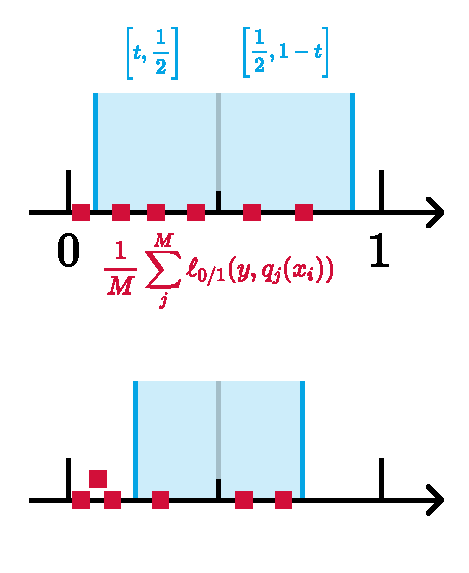
\includegraphics[width=0.8\textwidth]{competence}
  }
\end{frame}

\begin{frame}


\begin{align*}
\text{Weak learner:~~~}&\mathbb{E}_{(X,Y) }\left[ \Lzo{Y}{q_{\Theta}} \right] \geq \nicefrac{1}{2} \\[1.5em]
\text{$2$-competence:~~~}&
\forall t \in \left[ 0, \nicefrac{1}{2} \right]: ~ \prob{(X,Y) }{W \in \left[ t, \nicefrac{1}{2} \right]} ~ ~  \geq ~ ~ \prob{(X,Y) }{W \in \left[ \nicefrac{1}{2}, 1-t \right]}
\end{align*}

  \begin{theoremblock}{$\star$} 
The weak learner condition is a special case of $2$-competence
\end{theoremblock}
We have also in expectation
$$
\mathbb{E}_{\Theta,D}\left[ \mathbb{E}_{(X,Y) }\left[ \Lzo{Y}{\bar{q}} \right]  \right]  \geq \nicefrac{1}{2}
$$
Consequently,
\begin{align*}
\nicefrac{1}{2} &\leq \mathbb{E}_{\Theta,D, (X,Y) }\left[ \Lzo{Y}{\bar{q}} \right]  = \mathbb{E}_{(X,Y) }\left[ W \right]  \\
& ~\leftrightarrow~ \mathbb{E}_{(X,Y) }\left[ ~\ind{W \in \left[ 0, \nicefrac{1}{2} \right]}  \right] = \prob{(X,Y) }{W \in [0, \nicefrac{1}{2}]} = 1
\end{align*}

\end{frame}


\begin{frame}{Diversity and competence in binary classification problems}

  Assume $k=2$. Any vote that is not for class $y$ is automatically for the single other class.

  \begin{align*}
k = 2 ~\rightarrow~ 
\begin{cases}
W_{\Theta}  < \nicefrac{1}{2} ~\leftrightarrow~  \bar{q}(X) = Y \\[1em]
\compl{W_\Theta }  \leq \nicefrac{1}{2} ~\leftrightarrow~ \bar{q}(X) \not= Y
\end{cases}
\end{align*}

Starting from ambiguity decomp.:
\begin{theoremblock}{Lemma}
\begin{align*}
\mathbb{E}_{(X,Y) }\left[ \ell(Y, \bar{q}) \right]  &= \mathbb{E}_{(X,Y) , \Theta}\left[ \ell(Y, q) \right] - \mathbb{E}_{(X,Y) ,\Theta}\left[ \ell(Y, q) - \ell(Y, \bar{q}) \right] \\ 
&= \mathbb{E}_{(X,Y) ,\Theta}\left[ \ell(Y, q) \right] - \left(\mathbb{E}_{X_{+}}\left[ W_{\Theta}  \right] + \mathbb{E}_{X_{-}}\left[ W_{\Theta} -1 \right] \right) \\
&= \mathbb{E}_{(X,Y) ,\Theta}\left[ \ell(Y, q) \right] 
\underbrace{
- 
\mathbb{E}_{X_{+}}\left[ W_{\Theta}  \right] + \mathbb{E}_{X_{-}}\left[ 1-W_{\Theta} \right] 
}_{\text{diversity-effect for } k=2}
\end{align*}
\end{theoremblock}
where $X_{+}$ is range of $(X,Y)$ where $\bar{q}(X) = Y$ and $X_{-}$ vice versa.
Assume $Y=\bar{q}$, then $\Lzo{Y}{\bar{q}} = 0$ and diversity-effect becomes $W$.
Assume $Y \not= \bar{q}$, then diversity-effect becomes $\compl{W} - 1 = 1 - W$

\end{frame}

\begin{frame}
  Theisen et al. have shown that ($2$-competence) $\rightarrow$ (diversity-effect) $\geq 0$.
They established:
    \begin{align*}
  \text{$2$-competence} ~\leftrightarrow~ \mathbb{E}_{}\left[ W~\ind{W < \nicefrac{1}{2}} \right] \geq \mathbb{E}_{}\left[ 
  \compl{W}~\ind{\compl{W} \leq \nicefrac{1}{2} } 
  \right] 
  \end{align*}
  Consequently
  $$
d \defeq \mathbb{E}_{(X,Y),D }\left[ W_{\Theta} ~\ind{W_{\Theta} < \nicefrac{1}{2}} \right]  - \mathbb{E}_{(X,Y) ,D}\left[ \compl{W_{\Theta}} ~\ind{\compl{W_{\Theta}} \leq \nicefrac{1}{2} } \right] ~ ~ \geq ~ ~  0
$$
The indicator functions are mutually exclusive and can be understood as a case distinction. 
$$
d = 
\begin{cases}
\mathbb{E}_{X_+}\left[ W_{\Theta} \right] & \leftrightarrow W_{\Theta} < \nicefrac{1}{2} \\[1em]
\mathbb{E}_{X_-}\left[ \compl{W_{\Theta}}  \right]  = \mathbb{E}_{}\left[ 1 - W_{\Theta} \right]  & \leftrightarrow \compl{W_{\Theta}} \leq \nicefrac{1}{2} 
\end{cases}
$$
In binary classification, $d$ is nothing but diversity-effect. 

  \begin{theoremblock}{} $\star$ In binary classification problems, $2$-competence and non-negative diversity-effect are equivalent.
    $$
    k = 2 ~ ~ \Rightarrow ~ ~  \left( \text{$2$-competence} \leftrightarrow \text{diversity-effect}  \geq 0 \right)
    $$
  \end{theoremblock}

\end{frame}

\begin{frame}
  \frametitle{Competence and diversity in non-binary classification}
  \begin{itemize}
    \item For $k=2$, $\nicefrac{1}{2}$ is the classification threshold.
    \item For $k > 2$, $W \leq \nicefrac{1}{2}$ is sufficient but not necessary for correctness.
    \item Plurality vote can be won with less than $\nicefrac{1}{2}M$ votes.
  \end{itemize}
  Effective classification threshold for $k > 2$ is number of votes for next-best class. 
  \begin{definitionblock}{}
    $$
  \kappa (X,Y) = 1 - \max_{Z \not= Y} \mathbb{E}_{\Theta}\left[ ~\ind{q_{\Theta} = Z} \right] 
  $$
  \end{definitionblock}

  \begin{align*}
k \text{~arbitrary} ~\rightarrow ~
\begin{cases}
W_{\Theta} < \kappa  & ~\leftrightarrow~ \bar{q}(X) = Y \\[1.5em]
\compl{W_{\Theta}} \leq 1-\kappa &  ~\leftrightarrow~ \bar{q}(X) \not= Y
\end{cases}
\end{align*}

\begin{questionblock}{Claim}
  We can work with just \textit{some} classification threshold
\end{questionblock}

\end{frame}

\begin{frame}
  Recap: An ensemble is $2$-competent iff
  $$
  \forall t \in \left[ 0, \nicefrac{1}{2} \right]: ~ \prob{(X,Y) }{W \in \left[ t, \nicefrac{1}{2} \right]} ~ ~  \geq ~ ~ \prob{(X,Y) }{W \in \left[ \nicefrac{1}{2}, 1-t \right]}
  $$

  \begin{definitionblock}{$k$-competence}
        An ensemble is $k$-competent iff
$$
\forall t \in [0,1]:
\prob{(X,Y) }{W \in \left[ t, \kappa \right]}
\geq \prob{(X,Y) }{W \in \left[ 1-\kappa, 1-t \right]}
$$
for $ \kappa \defeq 1 - \max_{Z \not= Y} \mathbb{E}_{\Theta}\left[ ~\ind{q_{\Theta} = Z} \right]$.
  \end{definitionblock}
  \begin{theoremblock}{} $\star$ $2$-competence is a special case of $k$-competence in $2$-class problems.
\end{theoremblock}
We have seen that
$$
k= 2\text{:}  \hspace{1em} 2\text{-competence} ~\leftrightarrow~ ~ \text{diversity-effect}  \geq 0
$$
and we will show shortly that
$$
\text{diversity-effect} \geq 0 ~\leftrightarrow~ k\text{-competence} 
$$

\end{frame}
  
\begin{frame}
  Recap:
    \begin{align*}
  \text{$2$-competence} ~\leftrightarrow~ \mathbb{E}_{}\left[ W~\ind{W < \nicefrac{1}{2}} \right] \geq \mathbb{E}_{}\left[ 
  \compl{W}~\ind{\compl{W} \leq \nicefrac{1}{2} } 
  \right] 
  \end{align*}

  \begin{theoremblock}{Lemma} $\star$ It holds that
$$
\text{$k$-competence}  ~\leftrightarrow~ \mathbb{E}_{}\left[ W ~\ind{W < \kappa} \right] \geq \mathbb{E}_{}\left[ \compl{W} ~\ind{\compl{W} \leq \kappa } \right]  
$$
where $ \kappa \defeq 1 - \max_{Z \not= Y} \mathbb{E}_{\Theta}\left[ ~\ind{q_{\Theta} = Z} \right]$.
\end{theoremblock}
We begin by observing that, for all $x \in [0,1]$
% \begin{align*}
% & \prob{}{W \in [1-\kappa,1-x]} ~\ind{x \leq \kappa} \\
% =& \prob{}{W \in [1-\kappa,1-x ]} ~\ind{ 1-x > 1-\kappa } \\
% =& \prob{}{W ~\ind{W > 1-\kappa} ~ < ~ 1-x} \\
% =& \prob{}{W ~\ind{\compl{W} \leq \kappa } ~ < ~ 1-x} \\
% =& \prob{}{\compl{W} ~\ind{\compl{W} \leq \kappa } ~ \geq ~ x }
% \end{align*}
\begin{align*}
\prob{}{W \in [x, \kappa] } \cdot ~\ind{x \leq \kappa } &= \prob{}{W ~\ind{W < \kappa} ~ \geq ~ x} \\
\prob{}{W \in [1-\kappa,1-x]} \cdot ~\ind{x \leq \kappa} &= \prob{}{\compl{W} ~\ind{\compl{W} \leq \kappa } ~ \geq ~ x }
\end{align*}
where the first factors on the left-hand-side appear in the definition of $k$-competence.
Since $W$ is nonnegative, using that $\mathbb{E}_{}\left[ X \right] = \int \prob{}{X \geq x} \, dx$, we can conclude that, for any $x \in [0,1]$
\begin{align*}
\text{($k$-comp.)}  &~\leftrightarrow~  
\prob{}{W ~\ind{W < \kappa} ~ \geq x} 
~ ~ \geq ~ ~
\prob{}{\compl{W} ~\ind{\compl{W} \leq \kappa } ~ \geq x } \\
% & ~\leftrightarrow~
% \prob{}{f(W) ~\ind{W < \kappa} ~ \geq x} 
% ~ ~ \geq ~ ~
% \prob{}{f(\compl{W}) ~\ind{\compl{W} \leq \kappa } ~ \geq x } \\
& ~\leftrightarrow~
\mathbb{E}_{}\left[ W ~\ind{W < \kappa} \right] ~ ~ \geq ~ ~ \mathbb{E}_{}\left[ \compl{W} ~\ind{\compl{W} \leq \kappa }  \right] 
\end{align*}
\end{frame}

 \begin{frame}
\begin{theoremblock}{} $\star$ Consider an ensemble for a $k$-class classification problem. Then
$$
\text{$k$-competence}  ~ ~ ~\leftrightarrow~ ~ ~  \text{diversity-effect} \geq 0
$$
\end{theoremblock}
   \begin{align*}
        0 &= \mathbb{E}_{}\left[ (W-1)~\ind{W \geq \kappa} \right]  - \mathbb{E}_{}\left[ (W-1) ~\ind{W \geq \kappa} \right]  \\
        &= \mathbb{E}_{}\left[ (W-1)~\ind{W \geq \kappa} \right]  + \mathbb{E}_{}\left[ (1-W)~\ind{W \geq \kappa} \right]  \\
        &= \mathbb{E}_{}\left[ (W-1)~\ind{W \geq \kappa} \right]  + \mathbb{E}_{}\left[  \compl{W} ~\ind{\compl{W} < 1-\kappa} \right]   \\
        &\leq \mathbb{E}_{}\left[ (W-1)~\ind{W \geq \kappa} \right]  + \mathbb{E}_{}\left[  \compl{W} ~\ind{\compl{W} < \kappa} \right]   \\
    \end{align*}
Where the final inequality is enabled due to that, for $k \geq 2$, we have $\max_{Z \not= Y} \mathbb{E}_{\Theta}\left[ ~\ind{q_{\Theta} = Z} \right] < \nicefrac{1}{2}$ and consequently $\kappa \geq \nicefrac{1}{2}$ and $\kappa > 1-\kappa$.
    Applying the lemma to the second term yields
    % TODO need to make clearer that not only inequality holds but the gap actually *is* diversity-effect
    \begin{align*}
        & \mathbb{E}_{}\left[ (W-1)~\ind{W \geq \kappa} \right]  + \mathbb{E}_{}\left[  \compl{W} ~\ind{\compl{W} < \kappa} \right]   \\  
        \leq~ &  \mathbb{E}_{}\left[ (W-1)~\ind{W \geq \kappa} \right]  + \mathbb{E}_{}\left[ W ~\ind{W < \kappa} \right] 
    \end{align*}
 \end{frame} 

 \begin{frame}
    The above already is nothing but the diversity-effect:
    \begin{align*}
        0 \leq& \mathbb{E}_{}\left[ (W-1)~\ind{W \geq \kappa} \right]  + \mathbb{E}_{}\left[ W ~\ind{W < \kappa} \right]  \\
        = & \mathbb{E}_{}\left[ W  \right]  - \mathbb{E}_{}\left[ ~\ind{W \geq \kappa} \right]  \\
        = & \mathbb{E}_{}\left[ W \right]  - \prob{}{W \geq \kappa}
    \end{align*}
%     \marginnote{
%         \begin{align*}
% W \geq \kappa &~\leftrightarrow~ 1-t \\
% &~\leftrightarrow~ \compl{W}  = 1-W < t \\
% & ~\leftrightarrow~ \bar{q} = Y
% \end{align*}
%     }
    The first term is the ratio of incorrect members in expectation over all examples and is equal to the error rate of an average member. 
    The second term is the ensemble error. 
 \end{frame}


\begin{frame}

  \colandmargin{
 \begin{corollaryblock}{Note}
    Diversity is a measure of model fit (just like bias and variance)
  \end{corollaryblock}
  $\leadsto$ A more diverse ensemble is not necessarily better

  Nevertheless:

  \begin{questionblock}{Questions}
    \begin{itemize}
      \item Can we encourage diversity in Random Forests?
      \item Can we produce Random Forests with better generalisation error?
      \item Can we produce smaller forests?
    \end{itemize}
  \end{questionblock}

  We consider \zeroone-classification.
  }{
    \begin{figure}
        \includegraphics[width=0.7\textwidth]{symlinks/zero-one-plots/bvd-decomps/plot_bvd_standard_rf/mnist_subset/bvd-standard_rf.png}
  % \caption{
  %   Development of the \ensembleErrorCircle~ensemble error of a standard Random Forest ensemble as an increasing number of trees are added (evaluated on \textit{mnist} under \zeroone-loss). One can see that \avgBiasCircle~average member bias and \avgVarianceCircle~average member variance stay roughly equal while \diversityCircle~diversity increases, causing the ensemble error to decrease.
  % }
    \end{figure}
\begin{figure}
% \includegraphics[width=\textwidth]{symlinks/zero-one-plots/err_div/err_div/bioresponse/bvd-standard_rf.png}
\includegraphics[width=0.7\textwidth]{symlinks/zero-one-plots/err_div/err_div/qsar-biodeg/bvd-standard_rf.png}
\caption{
  Random Forests with varying number of trees plotted across average member error (vertical axis) and diversity (horizontal axis). 
}
\end{figure}
  }

\end{frame}

\begin{frame}

    Recall ambiguity-effect decomposition:
    $$
    \mathbb{E}_{}\left[ \Lzo{Y}{\bar{q}} \right] 
    = \mathbb{E}_{}\left[ \Lzo{Y}{q} \right]  - \mathbb{E}_{}\left[ \Lzo{Y}{q} - \Lzo{Y}{\bar{q}} \right] 
    $$
    For some point $(X,Y)$:
    \begin{itemize}
      \item Diversity term is positive (beneficial) if ensemble is correct
      \item Diversity term is negative (detrimental) if ensemble is incorrect
    \end{itemize}
    \textbf{Basic idea}: Encourage diversity on points where we can \textit{afford} diversity. (Increase "competence gap")

  \vspace{1em}
    Simple approach: 
    \begin{itemize}
      \item Example weights $w(X)$ $\leadsto$ will influence split search in DT construction
      \item Lower weight for $X$ $\leadsto$ higher average member error on $X$ $\leadsto$ higher diversity
    \end{itemize}

  \vspace{1em}
    \begin{itemize}
      \item Decision tree construction (implicitly) optimises a global loss function $\ell_{DT}$.
      \item Example weights correspond to "gradient descent in function space" ($\leadsto$ boosting).
    \end{itemize}

  \vspace{1em}
    Objective becomes
    $$
    \ell_{DT}(q(X),Y) - \lambda \cdot \ell_{\text{reg} }(q(X),Y)
    $$

    
\end{frame}

\begin{frame}

    \colandmargin{
      \begin{definitionblock}{ DRF weighting scheme  }
      Let $\bar{q}$ be the ensemble constructed so far. For a pair $(X,Y) \in D$, define the \textit{Dynamic Random Forest weighting scheme} as 
      $$
      w_{\text{DRF}}(X) \defeq W(X)
      \hspace{2em} \text{for~}  W(X) \defeq \Mavg \Lzo{Y}{q_i(X)}
      $$
      \label{def:drf-weighting-scheme}
      \end{definitionblock}
      $$
w_{\text{XuChen}}(X) \defeq \begin{cases}
W(X)^2 & \text{~if~} W(X) \leq \nicefrac{1}{2} \\ \\
\sqrt{W(X)} & \text{~if~} W(X) > \nicefrac{1}{2}
\end{cases}
$$
Note: only makes sense for binary classification (threshold at $\nicefrac{1}{2}$)

\vspace{1em}
    Two options to use weights:
    \begin{itemize}
      \item Weighted bootstrapping
      \item Weighted tree construction
    \end{itemize}
    }{
          \begin{figure}
          \includegraphics[width=0.8\textwidth]{weighting-fns/drf-fns.png}
    \caption{Illustration of \tikzcircle[fill=blue]{3pt}~$w_{\text{DRF}}$ and \tikzcircle[fill=orange]{3pt}~$w_{\text{XuChen}}$.}
          \end{figure}
    }

\end{frame}


\begin{frame}
    \begin{figure}
      
    \includegraphics[width=0.7\textwidth]{bvd-decomps/plot_bvd_drf/bvd.png}
    \caption{
        % Controlling $b$ sucessfullly mitigates spike but lower diversity for some reason. Capping then reaches higher diversity again. 
        % dvc-experiments/classification/zero-one/plots/bvd-decomps/plot_bvd_drf/bvd.png
         \bvdlegend
    }
    \end{figure}

\begin{corollaryblock}{}
    \begin{itemize}
        \item $w_\text{DRF}$ and $w_\text{XuChen}$ with weighted bootstrapping indeed lead to more diverse ensembles. For weighted tree construction, diversity is very similar to standard Random Forests.
        \item For weighted bootstrapping, there is an initial sharp increase in diversity and average member error. 
        \end{itemize}
\end{corollaryblock}
\end{frame}
  
\begin{frame}

  \begin{questionblock}{Claim}
    \begin{itemize}
      \item Incorrectly classified examples should not receive a higher weight 
      \begin{itemize}
        \item If anything, lower: subsequent correct votes will increase "bad" diversity (until majority vote is tipped)
      \end{itemize}
      \item Weighting function does not have to be linear.
    \end{itemize}
  \end{questionblock}

  \colandmargin{
\begin{definitionblock}{Sigmoid weighting function}
      \begin{align*}
    w_{\text{sigm} }(X) &\defeq \min\{ s, \nicefrac{1}{2} \} \\
    \text{for}~ ~ & s \defeq \text{sigmoid}(W(X) - t; 0, b, 1) \\
    & t \defeq \nicefrac{1}{2} \\
    & b \defeq b_\text{max}
    \end{align*}
    where the minimum clips the function values to a maximum of $\nicefrac{1}{2}$, $t = \nicefrac{1}{2}$ is the voting threshold.
\end{definitionblock}
\begin{definitionblock}{$w_\text{lerp}$}
  $$
  b \gets \frac{\min \{ M, M_{\text{max}} \}}{M_{\text{max} }} b_{\text{max} }
  $$
\end{definitionblock}

  }{
    \begin{figure}
          \includegraphics[width=\textwidth]{weighting-fns/sigmoid-fns.png}
    \caption{Illustration of \tcircle{orange}~$w_{\text{sigm}}$ for \tcircle{red}~$t = \nicefrac{1}{2}$ and varying $b$.}
    \end{figure}
  }

\end{frame}

\begin{frame}
      \begin{figure}
      \includegraphics[width=\textwidth]{symlinks/zero-one-plots/bvd-decomps/plot_bvd_capped_lerped_sigmoid/spambase-openml/bvd.png}
    \includegraphics[width=\textwidth]{symlinks/zero-one-plots/bvd-decomps/plot_bvd_capped_lerped_sigmoid/diabetes/bvd.png}
    \caption{
        Comparison of $w_\text{DRF}$, $w_\text{sigm}$ and $w_\text{lerp}$. \textit{diabetes} is a very small dataset with a high best achievable error rate.
        % Controlling $b$ sucessfullly mitigates spike but lower diversity for some reason. Capping then reaches higher diversity again. 
        % dvc-experiments/classification/zero-one/plots/bvd-decomps/plot_bvd_drf/bvd.png
    }
      \end{figure}

\begin{corollaryblock}{}
    \begin{itemize}
        \item Clipping (not assigning higher weights to incorrectly classified examples) already mitigates the spike in member error and diversity. Interpolating the steepness of the weighting function $b$ is not required for this. 
        \item Surprisingly, interpolating leads to higher diversity (sometimes even higher than $w_\text{DRF}$) and lower or similar ensemble generalisation error.
    \end{itemize}
\end{corollaryblock}
\end{frame}

\begin{frame}
  For non-binary classification problems:

  \colandmargin{
    \begin{definitionblock}{}
          $w_\text{dyn}$ is defined analogously to $w_\text{lerp}$, but $t$ is given as
          $$
          t \defeq \kappa(X,Y) = 1 - \max_{Z \not= Y} \mathbb{E}_{\Theta}\left[ ~\ind{q_{\Theta} = Z} \right] 
          $$
    \end{definitionblock}
  }{
    \begin{figure}
          \includegraphics[width=0.7\textwidth]{symlinks/illustrations/weighting-fns/sigmoid-fns-k.png}
    \end{figure}
  }
  \begin{figure}
    \includegraphics[width=\textwidth]{symlinks/zero-one-plots/bvd-decomps/plot_bvd_multiclass/digits/bvd.png}
    \caption{
        Comparison of $w_\text{lerp}$ and $w_\text{dyn}$ for a non-binary classification problem. 
    }
  \end{figure}
    \begin{corollaryblock}{}
     \begin{itemize}
        \item Using $w_\text{dyn}$, one can achieve slighly improvided ensemble generalisation error as compared to any other learner.
        \item The development of diversity is slower than with $w_\text{lerp}$ and more similar to standard Random Forests.
     \end{itemize}
  \end{corollaryblock}

\end{frame}
  
  
\begin{frame}

  \frametitle{Generalisation error for binary datasets}

  \colandmargin{
    \centering
    \includegraphics[width=21em]{ge-binary}
  }{
\begin{figure}
      \includegraphics[width=0.8\textwidth]{symlinks/zero-one-plots/compare_models/drf_sigmoid/spambase-openml/get_expected_ensemble_loss.png}
        \includegraphics[width=0.8\textwidth]{symlinks/zero-one-plots/compare_models/drf_sigmoid/diabetes/get_expected_ensemble_loss.png}
\end{figure}

  }

    % \begin{tabular}{llllll}%
    %  a b c d e f g
    % \csvreader[
    %     head=false
    % ]{.../written/thesis/symlinks/zero-one-plots/compare_models/drf_sigmoid/get_expected_ensemble_loss.csv}{}
    % % use head of csv as column names
    % {\\\hline
    % \csvcoli&
    % \csvcolii&
    % \csvcoliii&
    % \csvcoliv&
    % \csvcolv&
    % \csvcolvi
    % }% specify your coloumns here
    % \end{tabular}

\end{frame}

\begin{frame}
  \frametitle{Generalisation error for non-binary datasets}
  \colandmargin{
    \centering
    \includegraphics[width=20em]{ge-others}
  }{
\begin{figure}
      \includegraphics[width=0.8\textwidth]{symlinks/zero-one-plots/compare_models/dynamic_threshold/digits/get_expected_ensemble_loss.png}
\end{figure}
  }
\end{frame}






\begin{frame}

  \begin{itemize}
    \item[$\star$] Bias-Variance-Diversity decomposition from first principles 
  \item Bregman divergences vs. general loss functions and \zeroone-loss (non-negative vs good/bad diversity)
\item Weak learners and competence
\begin{itemize}
	\item Weak learners $~\rightarrow~$ $2$-competence
	\item[$\star$] $k=2 \Rightarrow$ $2$-competence $~\leftarrow~$ diversity-effect $\geq 0$ (equivalent)
	\item[$\star$]  $k=2$ $\Rightarrow$ $2$-competence $~\rightarrow~$ $k$-competence
	\item[$\star$]  $k$ arbitrary $\Rightarrow$ $k$-competence $~\leftrightarrow~$ diversity-effect $\geq 0$
\end{itemize}
\item Growth strategies
  \begin{itemize}
    \item Possible to encourage diversity in \zeroone-classification RFs
	\item Behaviour depends on datasets (error tradeoff; noise?)
	\item Possible to obtain better, smaller ensembles than standard RF
  \end{itemize}

  \end{itemize}
  \pause
    {
      \vspace{3em}
      \begin{center}
    Thanks for listening\\[1.15em]
     \Laughey[1.4] 
      \end{center}
    }
    % \includegraphics[width=1.5em]{laughey.png}
\end{frame}


\begin{frame}
 \frametitle{Effect decomps with noise} 

  % \frametitle{Noise, Bias and Variance}

  \colandmargin{
    \centering
    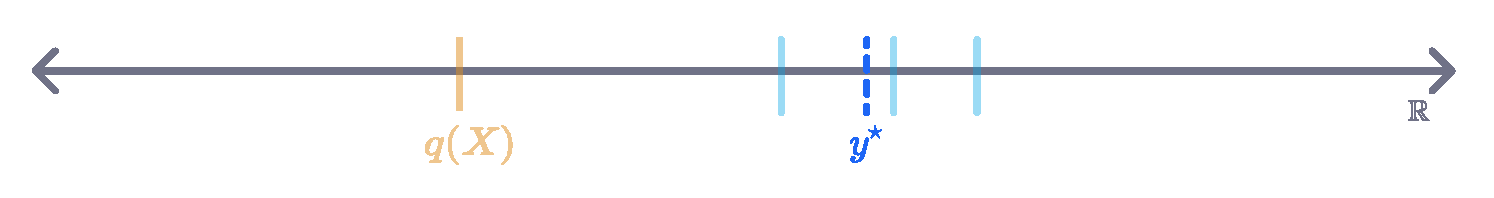
\includegraphics[width=\textwidth]{lnl-ambiguous-labels}
    {\small
    $ \mathbb{E}_{(X,Y)}\left[ \ell(Y, y^\star)\right]$ is \textit{noise}.
    }
  }{
  \begin{definitionblock}{Central Label}
    $$
    y^\star(X) \defeq \mathbb{E}_{Y \mid X}\left[Y\right]
    $$
  \end{definitionblock}
  }


  \colandmargin{
    \centering
    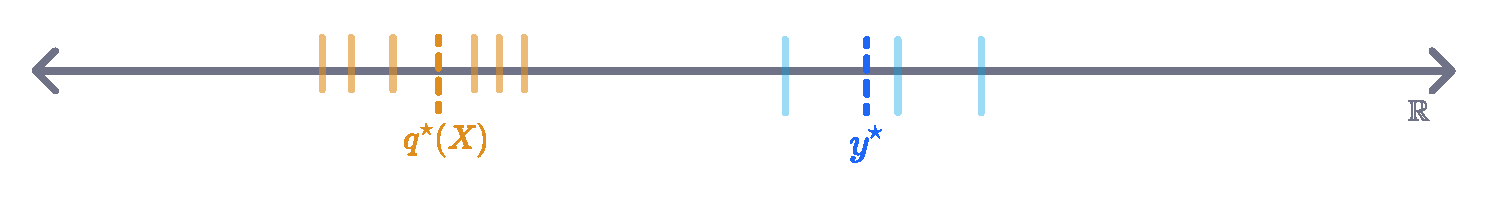
\includegraphics[width=\textwidth]{lnl-bias}
    {\small
    $\text{bias-effect}(X,Y) \defeq \ell(Y, q^\star) - \ell(Y, y^\star)$
    }
  }{
    \begin{definitionblock}{Central Model}
    $$
    q^\star \defeq \arg\min_{z} \mathbb{E}_{D}\left[ \ell(z, q_{D}) \right] 
    $$
    \end{definitionblock}
  }

  \colandmargin{
    \centering
    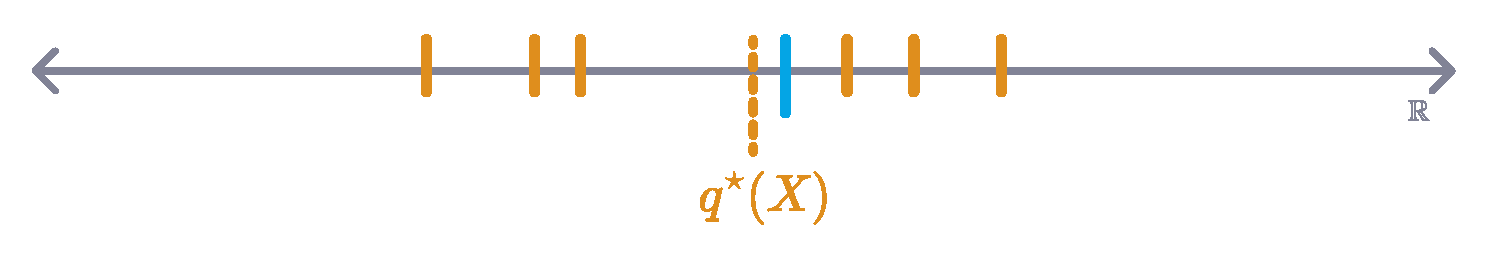
\includegraphics[width=\textwidth]{lnl-variance}
    {\small
    $\text{variance-effect}(X,Y) \defeq 
    \mathbb{E}_D \left[ \ell(Y, q_D)  \right] - \ell(Y, q^\star) 
    % =
    % \mathbb{E}_D \left[ \ell(Y, q_D) - \ell(Y, q^\star)   \right] 
    $
    }
  }{
    \small
    \begin{align*}
    \mathbb{E}_D \left[ \ell(Y, q_D)  \right] - \ell(Y, q^\star)  \\
    =
    \mathbb{E}_D \left[ \ell(Y, q_D) - \ell(Y, q^\star)   \right] 
    \end{align*}
  }


$$
\mathbb{E}_{}\left[ \ell(Y,q) \right]  = \mathbb{E}_{}\left[  
  % \underbrace{ 
    \ell(Y, y^\star) 
    % }_{\text{"noise"} }
+
% \underbrace{ 
  \ell(Y, q^\star) - \ell(Y, y^\star)
  %  }_{\text{"bias-effect"} }
+ 
% \underbrace{ 
  \ell(Y, q) - \ell(Y, q^\star) 
  % }_{\text{"variance-effect"} } 
  \right]
$$ 
\end{frame}
  
  
\end{document}